\chapter{Blender}

\section{Educational Game Development}
Educational games differ from other types of video games only in their
objective, that players learn as a result of playing. Educational games attempt
to take advantage of the engaging aspects of video game mechanics to entice
players into learning. It follows that improving the mechanics available for
creating video games will expand the toolset for creating educational games.


The most common elements of a video game include a two or three dimensional
environment which a player can manipulate. For many games the artistic
representation of the environment is important, as well as audio effects and
possibly interaction with other players over a network connection. Players must
be able to interact with the environment, often using a keyboard and mouse or a
specialized controller. The program which controls this environment and
provides the aforementioned functionality is generally referred to as a Game
Engine. Often times the resources which the Game Engine manipulates, such as
the artistic content and audio files are not created by the same program and
one must organize these resources and prepare them for use with the Game
Engine.


Currently there exist many free and non-free tools for creating video games,
including game engines, various two and three dimensional content creation
suites as well as audio and video editing programs. Professional game design
studios generally have teams of experts for each of these pieces of software
working together. An educator may not have these resources at their disposal and
thus it is desirable to seek a solution where most of the functionality can be
found in one program, thereby reducing the costs of learning and integrating
various components. Due to the relatively limited resources most educators have
access to, it is desirable to have a tool which is free to use. 


To these ends Blender \footnote{\url{http://www.blender.org}} was chosen as the basis for this project.
Blender is a powerful 3D content creation suite which has a built in Game
Engine. Blender has been in development for over a decade, with millions of
users world wide and a vibrant community of developers improving it daily.
Blender is an Open Source project, meaning that anyone is free to download the
source code and modify it. There is a large community of volunteers, students
who spend their summer funded by the Google Summer of Code initiative, as well
as full-time developers paid by the non-profit Blender Institute who
continually contribute code to the project. In addition to a development
community, there is a large community of users which post tutorials on Blenders
many features and several active mailing lists and forums where users give and
receive support for using Blender.



\section{Blender Game Engine}

The version of Blender used in this document is 2.57. The transition from
version 2.4x to 2.5x involved a complete overhaul of the User Interface as well
as many important internal changes which exclude the possibility of backwards
compatibility for games created in 2.5x.


The Blender Game Engine is tightly integrated with the Blender software, and
takes advantage of many of the content creation and 3D modeling features. The
starting point for any game is a Scene, which will usually contain various
Objects. These Objects can be manipulated in several ways by the game designer,
exposing them to interaction with the user, defining rules for physical
behavior or interaction with other Objects. The easiest way to create these
Objects is with the Blender interface which provides convenient methods for
constructing primitives as well as powerful tools for manipulating individual
vertices.


This section gives a brief overview of the core features of the Blender Game
Engine, many in depth tutorials and step-by-step tutorials are available for
free on the internet.


\subsection{Logic Editor}

The Logic Editor interface gives access to Game Properties and Logic bricks for
each Object in the Scene.  Logic bricks are the entry point for controlling
Objects in the Blender Game Engine, while Game Properties allow Objects to have
variables associated with them. Logic Bricks are divided into three classes:
Sensors, Controllers and Actuators.

\begin{figure}[!htc]
 		\centering
		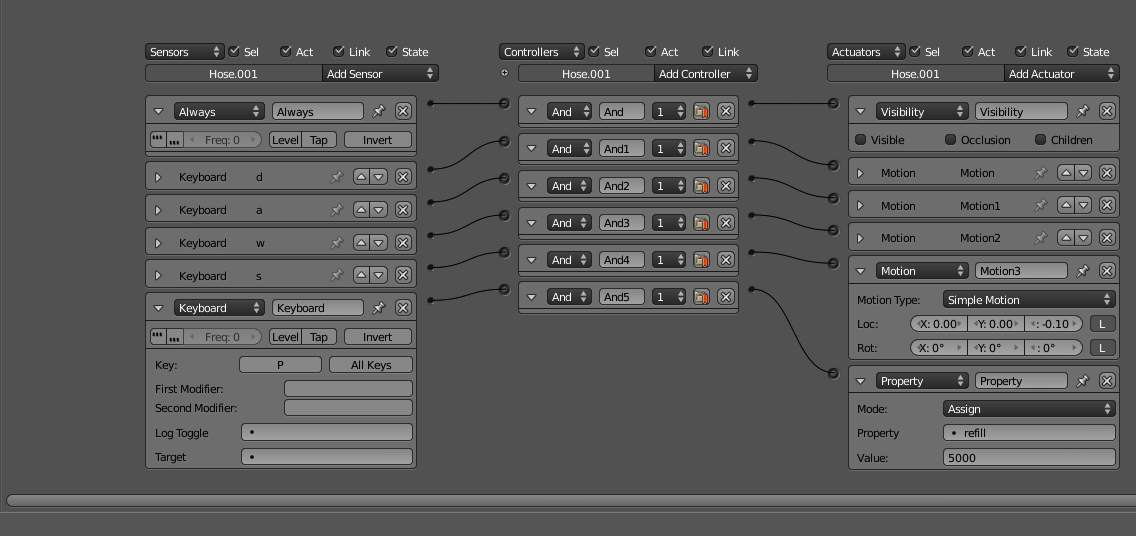
\includegraphics[scale=0.35]{figures/ui_logic.png}
        \caption{ Blender Game Engine Logic Bricks }
		\label{fig:logic}
\end{figure}


Sensors are how the Game Engine receives inputs, from the user as well as from
other objects or events. For example, to receive input from the keyboard one
would add a $Keyboard$ Sensor, or similarly a $Mouse$ Sensor. Other examples of
Sensors include collisions between Objects or the Always Sensor, which is
always active. The basic unit of time in the Game Engine is a frame,
so every frame each Sensor will be evaluated. If the Sensor is triggered it
will release an impulse to any Controllers it is attached to.


Controllers allow the game creator to combine the impulses from Sensors with
Boolean logic in order to decide what action will be taken upon the input. A
simple example would be to use an $And$ controller to determine if both the
$shift$ and $A$ keys have been pressed. If a controller is activated there are
two possible consequences, one or more Actuators are activated, or a Python
script is executed.


Actuators provide functionality for manipulating Objects such as moving or
rotating them, changing their properties or even destroying or adding new
Objects. While many interesting game functionalities can be realized using
actuators, any complex endeavor requires Python Scripting for practical
development.

\subsection{Python Scripting}
The Blender Game Engine, like the rest of the Blender software provides a
comprehensive Python scripting interface to the base functionality. Anything
possible with Logic Bricks is also possible with Python, with the added benefit
of extended functionality. Python scripts are used to make complex user
interfaces within games, manipulate objects and thier properties as well as
incorporate functionality from outside libraries.


\subsection{Physics}
Rigid body physical simulation is provided by the Bullet Physics library
\footnote{\url{http://bulletphysics.org}}. Rigid body physics allow for many interesting
effects and convincing interactions. 

The Blender software suite provides two fluid simulators, one developed as an
extension to Blender's particle system adn the other as an internal library.
Unfortunately neither of these fluid simulators is available in the game engine
since they are unable to perform at interactive speeds.



\subsection{Other Features}

The game engine includes a host of other features which can be utilized to
enhance a game but are not immediately relevant to this thesis. These features
include animations for controlling objects and characters, video textures for
playing video within a game, a networking module and support for a variety of
inputs. These features are continually being expanded in the core code as well as through
the addition of Python modules. 





